%设置页面边距（word标准页面）
\documentclass[a4paper]{article}
\usepackage{geometry}
\geometry{a4paper,left=2cm,right=2cm,top=1.6cm,bottom=1.6cm}

%导入ctex包
\usepackage[UTF8,heading=true]{ctex}

\usepackage{multirow}
\usepackage{amssymb}
\usepackage{amsmath}
\usepackage{float}
\usepackage{graphicx}
\usepackage{caption}
\captionsetup[figure]{labelsep=space}
\captionsetup[table]{labelsep=space,skip=2pt}
\ctexset {
    section = {
        name={,、},
        number=\chinese{section},
        aftername=,
        beforeskip=0.6em,
        afterskip=0.3em,
    },
}
\usepackage{booktabs}
\usepackage{enumitem}
\setlist{nosep,leftmargin=1.8em,topsep=1pt,parsep=0pt,itemsep=1pt}
\usepackage{fancyhdr}
\pagestyle{plain}
% 段落间距压紧
\setlength{\parskip}{2pt}
\linespread{1.05}

\title{\vspace{-2.5em}\Large\bfseries 2026 年信电学院电子设计竞赛\\大二 06 组 · 串口图像检测系统测试报告}
\date{}

\begin{document}
\maketitle
\vspace{-3em}
\zihao{5}

\section{院赛组号}
大二 06 组。

\section{系统整体架构框图}

\begin{center}
\begin{minipage}{0.98\textwidth}
\footnotesize
\begin{verbatim}
[PC 摄像头+JPG2COM] -- 灰度+JPEG(Q=90) --> [USB-TTL] -- UART 115200 8N1 -->
    +--------[纯模拟检测]---------+    +----------[STM32F103VE]----------+
    | LM324 积分/放大             |    | USART2(PA3)+DMA1_Ch6 环形收数    |
    | LM339 四档比较 -> 4 LED    |    | FF D8/FF D9 组帧 -> TJpgDec 解码 |
    +-----------------------------+    | 256 桶直方图 -> H, Hr           |
                                       | 4x 放大 -> FSMC -> ILI9341       |
                                       | H+L 闭眼检测 -> LED_RED+LCD 提示 |
                                       +----------------------------------+
\end{verbatim}
\end{minipage}
\end{center}

\section{电路原理图及简单说明}
\begin{figure}[H]
    \centering
    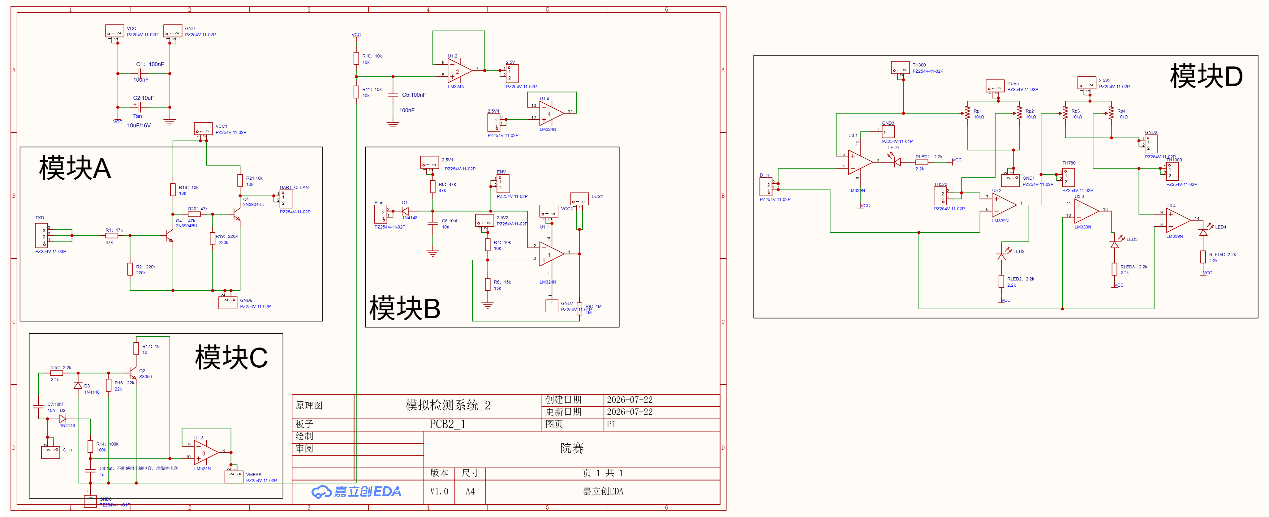
\includegraphics[width=0.8\textwidth]{resources/figure/circuit.png}
    \caption{电路原理图}
    \label{fig:circuit}
\end{figure}
电路独立于单片机工作，仅高阻采样 USB-TTL 模块的 TXD 信号，采用模块化设计：
\begin{itemize}
\item \textbf{电源与基准}：5\,V 供电 + 滤波去耦；电阻分压 + LM324 缓冲得约 2.5\,V 基准，供全电路使用。
\item \textbf{A · 信号整形}：TXD 经高阻电阻接 2N3904 共射极三极管，反相并整形为脉冲 UART\_CLEAN，采样电流小，对串口通信几乎无干扰。
\item \textbf{B · BUSY 生成}：UART\_CLEAN 经二极管 + RC 网络得包络 ENV；LM324 与基准做迟滞比较输出连续 BUSY 信号，其高电平持续时间 $\approx$ 一帧 JPEG 的串口发送时长。
\item \textbf{C · 帧长积分与保持}：BUSY 控制测量电容 C8 充电，把发送时长转成模拟电压 VMEAS；S8050 三极管在下一帧起始沿触发释放 C8，实现帧同步复位；LM324 电压跟随器缓冲 VMEAS 防止后级影响保持电压。
\item \textbf{D · 四档比较与显示}：VMEAS 同时送入 LM339 的四路比较器，四个 10\,k$\Omega$ 电位器分别设定 300 / 520 / 780 / 1000\,byte 附近阈值；四只 LED 采用累进式显示（1、2、3、4 只依次点亮）。
\end{itemize}

\section{基本部分完成情况}

LED 分级采用的比较阈值对应题目规定的四档文件帧长度区间。

\begin{table}[H]
\centering
\footnotesize
\caption{LED 分级理论对应关系与实测}
\begin{tabular}{cccc}
\toprule
等级 & 文件帧长度范围 (byte) & LED 显示  & 实测 LED 显示 \\
\midrule
1 & $300 < L \le 520$   & 亮灭灭灭 &  \\
2 & $520 < L \le 780$   & 亮亮灭灭 & \\
3 & $780 < L \le 1000$  & 亮亮亮灭  & \\
4 & $L > 1000$          & 亮亮亮亮  & \\
\bottomrule
\end{tabular}
\end{table}

从评测文件加载到 LED 稳定显示的时间间隔实测：\underline{\hspace{3em}} 秒。

\section{单片机方案（串口数据读取与 JPG 图像显示）}

采用的资源与实现要点：

\begin{itemize}
\item \textbf{串口}：USART2 (PA2/PA3, 115200 8N1) + DMA1 通道 6 循环模式常驻收数
（8 KB 环形缓冲）；20 ms 周期任务扫描 SOI (\texttt{FF D8}) / EOI (\texttt{FF D9})
完成组帧到 4 KB 单帧缓冲。
\item \textbf{JPG 解码}：TJpgDec 库，\texttt{JD\_FORMAT}=2 灰度直出，工作区 4.6 KB；
回调中同步累计 256 桶直方图。
\item \textbf{显示}：FSMC 并口驱动 ILI9341 (320$\times$240)；源图 48$\times$36 经
4$\times$ 最近邻放大得 192$\times$144，居中于屏幕上部；底部四行 8$\times$16 字体
信息区显示 H/Hr、帧率、闭眼状态。
\item \textbf{熵计算}：$H = -\sum_{i=0}^{255} p(i) \log_2 p(i)$，$H_r = H / 8$。
\end{itemize}

显示效果与精度测试（PC 端串口负载 0.8；PC = JPG2COM 面板读数，MCU = LCD 实测）：

\begin{table}[H]
\footnotesize
\centering
\caption{STM32 图像显示与熵值实测}
\begin{tabular}{|c|c|ccc|ccc|ccc|}
\hline
\multirow{2}{*}{测试图片} & \multirow{2}{*}{显示} & \multicolumn{3}{c|}{帧率 (fps)} & \multicolumn{3}{c|}{绝对熵 $H$} & \multicolumn{3}{c|}{相对熵 $H_r$} \\
\cline{3-11}
 &  & PC & MCU & 误差 & PC & MCU & 误差 & PC & MCU & 误差 \\
\hline
395-169\_54\_8   & 正常 & 21.0 & 15.7 & $-25.2\%$ & 1.350 & 1.613 & $+19.5\%$ & 0.169 & 0.202 & $+19.5\%$ \\
\hline
500-308\_66\_7   & 正常 & 16.0 & 16.0 & $0$       & 2.466 & 2.578 & $+4.5\%$  & 0.308 & 0.322 & $+4.5\%$ \\
\hline
620-410\_64\_9   & 正常 & 13.0 & 13.0 & $0$       & 3.282 & 3.369 & $+2.7\%$  & 0.410 & 0.421 & $+2.7\%$ \\
\hline
1186-738\_88\_4  & 正常 & 7.0  & 7.1  & $+1.4\%$  & 5.907 & 5.973 & $+1.1\%$  & 0.738 & 0.747 & $+1.2\%$ \\
\hline
realEye1         & 正常 & 7.0  & 7.1  & $+1.4\%$  & 6.340 & 6.360 & $+0.3\%$  & 0.793 & 0.795 & $+0.3\%$ \\
\hline
\end{tabular}
\end{table}

低熵图像上熵值偏差稍大，源于 TJpgDec 快速定点 IDCT 与 PC 端 libjpeg 高精度
IDCT 的 $\pm 1$ 灰度扰动，会在集中分布上产生若干新桶；高熵图像上差异可忽略。

\section{芯片使用统计}

\begin{table}[H]
\centering
\footnotesize
\caption{LM324 / LM339 数量统计}
\begin{tabular}{ccc}
\toprule
芯片型号 & 使用数量 & 用途 \\
\midrule
LM324 & 1 & 积分、信号调理放大 \\
LM339 & 1 & 四档窗口比较 \\
\bottomrule
\end{tabular}
\end{table}

\section{拓展完成情况}

\textbf{睁闭眼时文件帧大小变化}：睁眼时抠图区含虹膜/瞳孔与巩膜的高对比结构，
$L$ 处于高位（通常 $\ge$ 800 byte），LED 进入高档；闭眼时视野被眼皮/皮肤覆盖，
$L$ 落到 500\,--\,700 byte 区间，LED 进入低档。实测睁眼 $L \approx$
\underline{\hspace{2.5em}} byte，闭眼 $L \approx$ \underline{\hspace{2.5em}} byte。

\textbf{闭眼判断算法思路框架}：以每帧的绝对熵 $H$ 和 JPG 文件长度 $L$ 作为双
指标，四态迟滞状态机（\texttt{OPEN} $\to$ \texttt{MAYBE\_CLOSED} $\to$
\texttt{CLOSED} $\to$ \texttt{MAYBE\_OPEN} $\to$ \texttt{OPEN}）：

\begin{itemize}
\item 闭眼候选：$H < H_{\mathrm{ENTER}}$ \textbf{或} $L < L_{\mathrm{THR}}$；
\item 睁眼确认：$H \ge H_{\mathrm{EXIT}}$ \textbf{且} $L \ge L_{\mathrm{THR}}$；
\item 时间过滤：候选持续 $\ge T_{\mathrm{CLOSE}}$ 才判 CLOSED（过滤眨眼），
恢复需稳定 $\ge T_{\mathrm{OPEN}}$；
\item 输出：CLOSED 时点亮 LED\_RED (PB5) + LCD 显示 "EYE CLOSED"。
\end{itemize}

引入 $L$ 的原因：$H$ 为位置无关的全局直方图统计，对眼睛在抠图区的位置敏感、
闭眼时 $H$ 未必总能降到阈值以下；$L$ 反映压缩后信息量、位置耦合更弱，两者
 互补。默认参数：$H_{\mathrm{ENTER}}=6.35$ bit，$H_{\mathrm{EXIT}}=6.4$ bit，
$L_{\mathrm{THR}}=700$ byte，$T_{\mathrm{CLOSE}}=800$ ms，$T_{\mathrm{OPEN}}=300$ ms。

\textbf{测试结果}：闭眼确认延时 \underline{600\hspace{2.5em}} ms
\end{document}
